\newcommand{\ca}{\mathcal{A}}
\newcommand{\cb}{\mathcal{B}}
\renewcommand{\d}{\Delta}

%% bare_jrnl.tex
%% V1.4b
%% 2015/08/26
%% by Michael Shell
%% see http://www.michaelshell.org/
%% for current contact information.
%%
%% This is a skeleton file demonstrating the use of IEEEtran.cls
%% (requires IEEEtran.cls version 1.8b or later) with an IEEE
%% journal paper.
%%
%% Support sites:
%% http://www.michaelshell.org/tex/ieeetran/
%% http://www.ctan.org/pkg/ieeetran
%% and
%% http://www.ieee.org/

%%*************************************************************************
%% Legal Notice:
%% This code is offered as-is without any warranty either expressed or
%% implied; without even the implied warranty of MERCHANTABILITY or
%% FITNESS FOR A PARTICULAR PURPOSE! 
%% User assumes all risk.
%% In no event shall the IEEE or any contributor to this code be liable for
%% any damages or losses, including, but not limited to, incidental,
%% consequential, or any other damages, resulting from the use or misuse
%% of any information contained here.
%%
%% All comments are the opinions of their respective authors and are not
%% necessarily endorsed by the IEEE.
%%
%% This work is distributed under the LaTeX Project Public License (LPPL)
%% ( http://www.latex-project.org/ ) version 1.3, and may be freely used,
%% distributed and modified. A copy of the LPPL, version 1.3, is included
%% in the base LaTeX documentation of all distributions of LaTeX released
%% 2003/12/01 or later.
%% Retain all contribution notices and credits.
%% ** Modified files should be clearly indicated as such, including  **
%% ** renaming them and changing author support contact information. **
%%*************************************************************************


% *** Authors should verify (and, if needed, correct) their LaTeX system  ***
% *** with the testflow diagnostic prior to trusting their LaTeX platform ***
% *** with production work. The IEEE's font choices and paper sizes can   ***
% *** trigger bugs that do not appear when using other class files.       ***                          ***
% The testflow support page is at:
% http://www.michaelshell.org/tex/testflow/


% Please refer to your journal's instructions for other
% options that should be set.
\documentclass[journal,onecolumn]{IEEEtran}
%
% If IEEEtran.cls has not been installed into the LaTeX system files,
% manually specify the path to it like:
% \documentclass[journal]{../sty/IEEEtran}





% Some very useful LaTeX packages include:
% (uncomment the ones you want to load)


% *** MISC UTILITY PACKAGES ***
%
%\usepackage{ifpdf}
% Heiko Oberdiek's ifpdf.sty is very useful if you need conditional
% compilation based on whether the output is pdf or dvi.
% usage:
% \ifpdf
%   % pdf code
% \else
%   % dvi code
% \fi
% The latest version of ifpdf.sty can be obtained from:
% http://www.ctan.org/pkg/ifpdf
% Also, note that IEEEtran.cls V1.7 and later provides a builtin
% \ifCLASSINFOpdf conditional that works the same way.
% When switching from latex to pdflatex and vice-versa, the compiler may
% have to be run twice to clear warning/error messages.






% *** CITATION PACKAGES ***
%
\usepackage{cite}
% cite.sty was written by Donald Arseneau
% V1.6 and later of IEEEtran pre-defines the format of the cite.sty package
% \cite{} output to follow that of the IEEE. Loading the cite package will
% result in citation numbers being automatically sorted and properly
% "compressed/ranged". e.g., [1], [9], [2], [7], [5], [6] without using
% cite.sty will become [1], [2], [5]--[7], [9] using cite.sty. cite.sty's
% \cite will automatically add leading space, if needed. Use cite.sty's
% noadjust option (cite.sty V3.8 and later) if you want to turn this off
% such as if a citation ever needs to be enclosed in parenthesis.
% cite.sty is already installed on most LaTeX systems. Be sure and use
% version 5.0 (2009-03-20) and later if using hyperref.sty.
% The latest version can be obtained at:
% http://www.ctan.org/pkg/cite
% The documentation is contained in the cite.sty file itself.






% *** GRAPHICS RELATED PACKAGES ***
%
\ifCLASSINFOpdf
	\usepackage[pdftex]{graphicx}
	% declare the path(s) where your graphic files are
	% \graphicspath{{./Code/}{.}}
	% and their extensions so you won't have to specify these with
	% every instance of \includegraphics
	\DeclareGraphicsExtensions{.pdf,.jpeg,.png,.jpg}
\else
	% or other class option (dvipsone, dvipdf, if not using dvips). graphicx
	% will default to the driver specified in the system graphics.cfg if no
	% driver is specified.
	% \usepackage[dvips]{graphicx}
	% declare the path(s) where your graphic files are
	% \graphicspath{{../eps/}}
	% and their extensions so you won't have to specify these with
	% every instance of \includegraphics
	% \DeclareGraphicsExtensions{.eps}
\fi
% graphicx was written by David Carlisle and Sebastian Rahtz. It is
% required if you want graphics, photos, etc. graphicx.sty is already
% installed on most LaTeX systems. The latest version and documentation
% can be obtained at: 
% http://www.ctan.org/pkg/graphicx
% Another good source of documentation is "Using Imported Graphics in
% LaTeX2e" by Keith Reckdahl which can be found at:
% http://www.ctan.org/pkg/epslatex
%
% latex, and pdflatex in dvi mode, support graphics in encapsulated
% postscript (.eps) format. pdflatex in pdf mode supports graphics
% in .pdf, .jpeg, .png and .mps (metapost) formats. Users should ensure
% that all non-photo figures use a vector format (.eps, .pdf, .mps) and
% not a bitmapped formats (.jpeg, .png). The IEEE frowns on bitmapped formats
% which can result in "jaggedy"/blurry rendering of lines and letters as
% well as large increases in file sizes.
%
% You can find documentation about the pdfTeX application at:
% http://www.tug.org/applications/pdftex





% *** MATH PACKAGES ***
%
\usepackage{amsmath}
% A popular package from the American Mathematical Society that provides
% many useful and powerful commands for dealing with mathematics.
%
% Note that the amsmath package sets \interdisplaylinepenalty to 10000
% thus preventing page breaks from occurring within multiline equations. Use:
\interdisplaylinepenalty=2500
% after loading amsmath to restore such page breaks as IEEEtran.cls normally
% does. amsmath.sty is already installed on most LaTeX systems. The latest
% version and documentation can be obtained at:
% http://www.ctan.org/pkg/amsmath





% *** SPECIALIZED LIST PACKAGES ***
%
\usepackage{algorithmic}
% algorithmic.sty was written by Peter Williams and Rogerio Brito.
% This package provides an algorithmic environment for describing algorithms.
% You can use the algorithmic environment in-text or within a figure
% environment to provide for a floating algorithm. Do NOT use the algorithm
% floating environment provided by algorithm.sty (by the same authors) or
% algorithm2e.sty (by Christophe Fiorio) as the IEEE does not use dedicated
% algorithm float types and packages that provide these will not provide
% correct IEEE style captions. The latest version and documentation of
% algorithmic.sty can be obtained at:
% http://www.ctan.org/pkg/algorithms
% Also of interest may be the (relatively newer and more customizable)
% algorithmicx.sty package by Szasz Janos:
% http://www.ctan.org/pkg/algorithmicx




% *** ALIGNMENT PACKAGES ***
%
\usepackage{array}
% Frank Mittelbach's and David Carlisle's array.sty patches and improves
% the standard LaTeX2e array and tabular environments to provide better
% appearance and additional user controls. As the default LaTeX2e table
% generation code is lacking to the point of almost being broken with
% respect to the quality of the end results, all users are strongly
% advised to use an enhanced (at the very least that provided by array.sty)
% set of table tools. array.sty is already installed on most systems. The
% latest version and documentation can be obtained at:
% http://www.ctan.org/pkg/array


% IEEEtran contains the IEEEeqnarray family of commands that can be used to
% generate multiline equations as well as matrices, tables, etc., of high
% quality.




% *** SUBFIGURE PACKAGES ***
\ifCLASSOPTIONcompsoc
	\usepackage[caption=false,font=normalsize,labelfont=sf,textfont=sf]{subfig}
\else
	\usepackage[caption=false,font=footnotesize]{subfig}
\fi
% subfig.sty, written by Steven Douglas Cochran, is the modern replacement
% for subfigure.sty, the latter of which is no longer maintained and is
% incompatible with some LaTeX packages including fixltx2e. However,
% subfig.sty requires and automatically loads Axel Sommerfeldt's caption.sty
% which will override IEEEtran.cls' handling of captions and this will result
% in non-IEEE style figure/table captions. To prevent this problem, be sure
% and invoke subfig.sty's "caption=false" package option (available since
% subfig.sty version 1.3, 2005/06/28) as this is will preserve IEEEtran.cls
% handling of captions.
% Note that the Computer Society format requires a larger sans serif font
% than the serif footnote size font used in traditional IEEE formatting
% and thus the need to invoke different subfig.sty package options depending
% on whether compsoc mode has been enabled.
%
% The latest version and documentation of subfig.sty can be obtained at:
% http://www.ctan.org/pkg/subfig




% *** FLOAT PACKAGES ***
%
%\usepackage{fixltx2e}
% fixltx2e, the successor to the earlier fix2col.sty, was written by
% Frank Mittelbach and David Carlisle. This package corrects a few problems
% in the LaTeX2e kernel, the most notable of which is that in current
% LaTeX2e releases, the ordering of single and double column floats is not
% guaranteed to be preserved. Thus, an unpatched LaTeX2e can allow a
% single column figure to be placed prior to an earlier double column
% figure.
% Be aware that LaTeX2e kernels dated 2015 and later have fixltx2e.sty's
% corrections already built into the system in which case a warning will
% be issued if an attempt is made to load fixltx2e.sty as it is no longer
% needed.
% The latest version and documentation can be found at:
% http://www.ctan.org/pkg/fixltx2e


%\usepackage{stfloats}
% stfloats.sty was written by Sigitas Tolusis. This package gives LaTeX2e
% the ability to do double column floats at the bottom of the page as well
% as the top. (e.g., "\begin{figure*}[!b]" is not normally possible in
% LaTeX2e). It also provides a command:
%\fnbelowfloat
% to enable the placement of footnotes below bottom floats (the standard
% LaTeX2e kernel puts them above bottom floats). This is an invasive package
% which rewrites many portions of the LaTeX2e float routines. It may not work
% with other packages that modify the LaTeX2e float routines. The latest
% version and documentation can be obtained at:
% http://www.ctan.org/pkg/stfloats
% Do not use the stfloats baselinefloat ability as the IEEE does not allow
% \baselineskip to stretch. Authors submitting work to the IEEE should note
% that the IEEE rarely uses double column equations and that authors should try
% to avoid such use. Do not be tempted to use the cuted.sty or midfloat.sty
% packages (also by Sigitas Tolusis) as the IEEE does not format its papers in
% such ways.
% Do not attempt to use stfloats with fixltx2e as they are incompatible.
% Instead, use Morten Hogholm'a dblfloatfix which combines the features
% of both fixltx2e and stfloats:
%
% \usepackage{dblfloatfix}
% The latest version can be found at:
% http://www.ctan.org/pkg/dblfloatfix




%\ifCLASSOPTIONcaptionsoff
%  \usepackage[nomarkers]{endfloat}
% \let\MYoriglatexcaption\caption
% \renewcommand{\caption}[2][\relax]{\MYoriglatexcaption[#2]{#2}}
%\fi
% endfloat.sty was written by James Darrell McCauley, Jeff Goldberg and 
% Axel Sommerfeldt. This package may be useful when used in conjunction with 
% IEEEtran.cls'  captionsoff option. Some IEEE journals/societies require that
% submissions have lists of figures/tables at the end of the paper and that
% figures/tables without any captions are placed on a page by themselves at
% the end of the document. If needed, the draftcls IEEEtran class option or
% \CLASSINPUTbaselinestretch interface can be used to increase the line
% spacing as well. Be sure and use the nomarkers option of endfloat to
% prevent endfloat from "marking" where the figures would have been placed
% in the text. The two hack lines of code above are a slight modification of
% that suggested by in the endfloat docs (section 8.4.1) to ensure that
% the full captions always appear in the list of figures/tables - even if
% the user used the short optional argument of \caption[]{}.
% IEEE papers do not typically make use of \caption[]'s optional argument,
% so this should not be an issue. A similar trick can be used to disable
% captions of packages such as subfig.sty that lack options to turn off
% the subcaptions:
% For subfig.sty:
% \let\MYorigsubfloat\subfloat
% \renewcommand{\subfloat}[2][\relax]{\MYorigsubfloat[]{#2}}
% However, the above trick will not work if both optional arguments of
% the \subfloat command are used. Furthermore, there needs to be a
% description of each subfigure *somewhere* and endfloat does not add
% subfigure captions to its list of figures. Thus, the best approach is to
% avoid the use of subfigure captions (many IEEE journals avoid them anyway)
% and instead reference/explain all the subfigures within the main caption.
% The latest version of endfloat.sty and its documentation can obtained at:
% http://www.ctan.org/pkg/endfloat
%
% The IEEEtran \ifCLASSOPTIONcaptionsoff conditional can also be used
% later in the document, say, to conditionally put the References on a 
% page by themselves.




% *** PDF, URL AND HYPERLINK PACKAGES ***
%
\usepackage{url}
% url.sty was written by Donald Arseneau. It provides better support for
% handling and breaking URLs. url.sty is already installed on most LaTeX
% systems. The latest version and documentation can be obtained at:
% http://www.ctan.org/pkg/url
% Basically, \url{my_url_here}.




% *** Do not adjust lengths that control margins, column widths, etc. ***
% *** Do not use packages that alter fonts (such as pslatex).         ***
% There should be no need to do such things with IEEEtran.cls V1.6 and later.
% (Unless specifically asked to do so by the journal or conference you plan
% to submit to, of course. )


% correct bad hyphenation here
\hyphenation{op-tical net-works semi-conduc-tor}


\begin{document}
%
% paper title
% Titles are generally capitalized except for words such as a, an, and, as,
% at, but, by, for, in, nor, of, on, or, the, to and up, which are usually
% not capitalized unless they are the first or last word of the title.
% Linebreaks \\ can be used within to get better formatting as desired.
% Do not put math or special symbols in the title.
\title{Fundamentals of Wave Simulation: \\ Source Terms}
%
%
% author names and IEEE memberships
% note positions of commas and nonbreaking spaces ( ~ ) LaTeX will not break
% a structure at a ~ so this keeps an author's name from being broken across
% two lines.
% use \thanks{} to gain access to the first footnote area
% a separate \thanks must be used for each paragraph as LaTeX2e's \thanks
% was not built to handle multiple paragraphs
%

%\author{Michael~Shell,~\IEEEmembership{Member,~IEEE,}
%        John~Doe,~\IEEEmembership{Fellow,~OSA,}
%        and~Jane~Doe,~\IEEEmembership{Life~Fellow,~IEEE}% <-this % stops a space
%\thanks{M. Shell was with the Department
%of Electrical and Computer Engineering, Georgia Institute of Technology, Atlanta,
%GA, 30332 USA e-mail: (see http://www.michaelshell.org/contact.html).}% <-this % stops a space
%\thanks{J. Doe and J. Doe are with Anonymous University.}% <-this % stops a space
%\thanks{Manuscript received April 19, 2005; revised August 26, 2015.}}
\author{Matilde Tozzi}

% note the % following the last \IEEEmembership and also \thanks - 
% these prevent an unwanted space from occurring between the last author name
% and the end of the author line. i.e., if you had this:
% 
% \author{....lastname \thanks{...} \thanks{...} }
%                     ^------------^------------^----Do not want these spaces!
%
% a space would be appended to the last name and could cause every name on that
% line to be shifted left slightly. This is one of those "LaTeX things". For
% instance, "\textbf{A} \textbf{B}" will typeset as "A B" not "AB". To get
% "AB" then you have to do: "\textbf{A}\textbf{B}"
% \thanks is no different in this regard, so shield the last } of each \thanks
% that ends a line with a % and do not let a space in before the next \thanks.
% Spaces after \IEEEmembership other than the last one are OK (and needed) as
% you are supposed to have spaces between the names. For what it is worth,
% this is a minor point as most people would not even notice if the said evil
% space somehow managed to creep in.



% The paper headers
%\markboth{Journal of \LaTeX\ Class Files,~Vol.~14, No.~8, August~2015}%
%{Shell \MakeLowercase{\textit{et al.}}: Bare Demo of IEEEtran.cls for IEEE Journals}
% The only time the second header will appear is for the odd numbered pages
% after the title page when using the twoside option.
% 
% *** Note that you probably will NOT want to include the author's ***
% *** name in the headers of peer review papers.                   ***
% You can use \ifCLASSOPTIONpeerreview for conditional compilation here if
% you desire.




% If you want to put a publisher's ID mark on the page you can do it like
% this:
%\IEEEpubid{0000--0000/00\$00.00~\copyright~2015 IEEE}
% Remember, if you use this you must call \IEEEpubidadjcol in the second
% column for its text to clear the IEEEpubid mark.



% use for special paper notices
%\IEEEspecialpapernotice{(Invited Paper)}




% make the title area
\maketitle

% As a general rule, do not put math, special symbols or citations
% in the abstract or keywords.
\begin{abstract}
	The abstract goes here.
\end{abstract}

% Note that keywords are not normally used for peerreview papers.
\begin{IEEEkeywords}
	Wave Simulation, Source Terms, Seminar, PDE, ODE, Fractional Methods.
\end{IEEEkeywords}






% For peer review papers, you can put extra information on the cover
% page as needed:
% \ifCLASSOPTIONpeerreview
% \begin{center} \bfseries EDICS Category: 3-BBND \end{center}
% \fi
%
% For peerreview papers, this IEEEtran command inserts a page break and
% creates the second title. It will be ignored for other modes.
\IEEEpeerreviewmaketitle

% The very first letter is a 2 line initial drop letter followed
% by the rest of the first word in caps.
% 
% form to use if the first word consists of a single letter:
% \IEEEPARstart{A}{demo} file is ....
% 
% Some journals put the first two words in caps:
% \IEEEPARstart{T}{his demo} file is ....
% 
% Here we have the typical use of a "T" for an initial drop letter
% and "HIS" in caps to complete the first word.
\section {Introduction}

\IEEEPARstart{M}{ost} of the content of this paper (and the mathematical notation) is from \cite{leveque}. The code is my own and can be found in \cite{github}. I try to use Julia as an exercise. I also took inspiration from \cite {clawpack} and \cite {riemann}.

\section{From Conservation Laws to Balance Laws}
In this paper, we examine some numerical methods for the solution of \textit{non homogeneous balance laws}. These are an extension of the well-known \textit{conservation laws} of the form $q_t+f(q)_x=0$ by adding a \textit{source term} $\psi(q)$. This is called source term even if physically it represents a sink rather than a source, i.e. a loss of $q$. Our reference equation is therefore

\begin{equation} \label{eq:template}
	q_t + f(q)_x = \psi(q).
\end{equation}

We will mostly study problems where the homogeneous equation

\begin{equation} \label{eq:hom}
	q_t +f(q)_x = 0
\end{equation}

is \textit{hyperbolic} and the source terms don't depend on derivatives of $q$, so that

\begin{equation} \label{eq:source}
	q_t = \psi(q)
\end{equation}

is an independent system of ODEs.




% needed in second column of first page if using \IEEEpubid
%\IEEEpubidadjcol




% An example of a floating figure using the graphicx package.
% Note that \label must occur AFTER (or within) \caption.
% For figures, \caption should occur after the \includegraphics.
% Note that IEEEtran v1.7 and later has special internal code that
% is designed to preserve the operation of \label within \caption
% even when the captionsoff option is in effect. However, because
% of issues like this, it may be the safest practice to put all your
% \label just after \caption rather than within \caption{}.
%
% Reminder: the "draftcls" or "draftclsnofoot", not "draft", class
% option should be used if it is desired that the figures are to be
% displayed while in draft mode.
%
% \begin{figure}[!ht]
% 	\centering
% 	\includegraphics[width=2.5in]{bears}
% 	% where an .eps filename suffix will be assumed under latex, 
% 	% and a .pdf suffix will be assumed for pdflatex; or what has been declared
% 	% via \DeclareGraphicsExtensions.
% 	\caption{Simulation results for the network.}
% 	\label{fig_sim}
% \end{figure}

% Note that the IEEE typically puts floats only at the top, even when this
% results in a large percentage of a column being occupied by floats.


% An example of a double column floating figure using two subfigures.
% (The subfig.sty package must be loaded for this to work.)
% The subfigure \label commands are set within each subfloat command,
% and the \label for the overall figure must come after \caption.
% \hfil is used as a separator to get equal spacing.
% Watch out that the combined width of all the subfigures on a 
% line do not exceed the text width or a line break will occur.
%
% \begin{figure*}[!ht]
% 	\centering
% 	\subfloat[Case I]{\includegraphics[width=2.5in]{bears}%
% 		\label{fig_first_case}}
% 	\hfil
% 	\subfloat[Case II]{\includegraphics[width=2.5in]{tree}%
% 		\label{fig_second_case}}
% 	\caption{Simulation results for the network.}
% 	\label{fig_sim2}
% \end{figure*}
%
% Note that often IEEE papers with subfigures do not employ subfigure
% captions (using the optional argument to \subfloat[]), but instead will
% reference/describe all of them (a), (b), etc., within the main caption.
% Be aware that for subfig.sty to generate the (a), (b), etc., subfigure
% labels, the optional argument to \subfloat must be present. If a
% subcaption is not desired, just leave its contents blank,
% e.g., \subfloat[].


% An example of a floating table. Note that, for IEEE style tables, the
% \caption command should come BEFORE the table and, given that table
% captions serve much like titles, are usually capitalized except for words
% such as a, an, and, as, at, but, by, for, in, nor, of, on, or, the, to
% and up, which are usually not capitalized unless they are the first or
% last word of the caption. Table text will default to \footnotesize as
% the IEEE normally uses this smaller font for tables.
% The \label must come after \caption as always.
%
%\begin{table}[!t]
%% increase table row spacing, adjust to taste
%\renewcommand{\arraystretch}{1.3}
% if using array.sty, it might be a good idea to tweak the value of
% \extrarowheight as needed to properly center the text within the cells
%\caption{An Example of a Table}
%\label{table_example}
%\centering
%% Some packages, such as MDW tools, offer better commands for making tables
%% than the plain LaTeX2e tabular which is used here.
%\begin{tabular}{|c||c|}
%\hline
%One & Two\\
%\hline
%Three & Four\\
%\hline
%\end{tabular}
%\end{table}


% Note that the IEEE does not put floats in the very first column
% - or typically anywhere on the first page for that matter. Also,
% in-text middle ("here") positioning is typically not used, but it
% is allowed and encouraged for Computer Society conferences (but
% not Computer Society journals). Most IEEE journals/conferences use
% top floats exclusively. 
% Note that, LaTeX2e, unlike IEEE journals/conferences, places
% footnotes above bottom floats. This can be corrected via the
% \fnbelowfloat command of the stfloats package.




\section{Godunov-Strang splitting}

One standard approach to these problems is using a \textit{fractional-step} or \textit{operator-splitting} method, where we alternate between solving the homogeneous \eqref{eq:hom} and source \eqref{eq:source} term. This allows us to easily use a lot of standard numerical methods for PDEs and ODEs.

\subsection{The Advection-Reaction Equation}

The standard example that will be used to illustrate all the following numerical methods is the \textit{advection-reaction} equation, which can be seen as the model for the transport along a flow of a radioactive substance which decays at rate $\beta$ while it's transported at constant speed $\bar{u}$, with initial data $q(x,0)= \mathring{q}(x)$.

\begin{equation}\label{eq:advec}
	q_t + \bar{u}q_x=-\beta q
\end{equation}

We can compute the exact solution of \eqref{eq:advec}, because along the characteristic $\frac{dx}{dt}=\bar{u}$ we have $\frac{dq}{dt}=-\beta q$ and it follows that

\begin{equation}\label{eq:advec_sol}
	q(x,t) = e^{-\beta t}\mathring{q}(x-\bar{u}t).
\end{equation}

\begin{figure}[!ht]
	\centering
	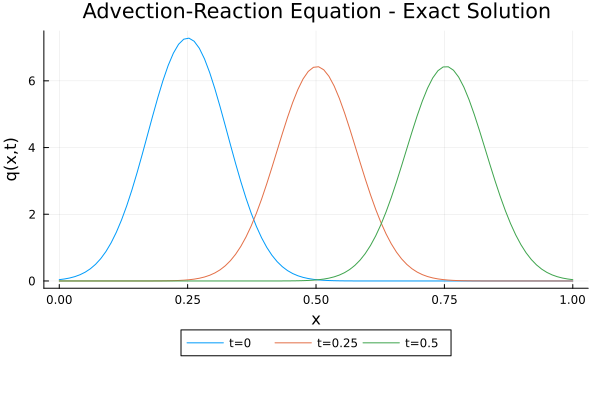
\includegraphics[width=0.5\textwidth]{Advection.png}
	% where an .eps filename suffix will be assumed under latex, 
	% and a .pdf suffix will be assumed for pdflatex; or what has been declared
	% via \DeclareGraphicsExtensions.
	\caption{Evolution of the exact solution with $\bar{u}=1$, $\beta=1$, and $\mathring{q}=\text{Gaussian}(0.25,0.003)$. We see that the maximum point decreases in time.}
	\label{fig:exact}
\end{figure}

\subsection{The Unsplit Method}

Of course for this specific example we can easily compute an \textit{unsplit} method

\begin{equation}\label{eq:unsplit}
	\frac{Q^{n+1}_i-Q^n_i}{\d t} = -\bar{u} \frac{Q^n_i-Q^n_{i-1}}{\d x}-\beta Q^n_i \Rightarrow Q^{n+1}_i = Q^n_i-\bar{u} \frac{\d t}{\d x}(Q^n_i-Q^n_{i-1})-\d t\beta Q^n_i
\end{equation}

which is first-order accurate and stable for $0<\bar{u}\frac{\d t}{\d x}\leq1$.
A second-order method is also easily obtainable with the Taylor expansion of $q(x,t+\d t)$ as explained in \cite{leveque}. An important thing to note is that the full Taylor expansion of \eqref{eq:advec} can be written formally as

\begin{equation}\label{eq:sol_op}
	e^{-\d t(\bar{u}\partial_x+\beta)}q(x,t):=q(x,t+\d t)=\sum_{j=0}^{\infty}\frac{(\d t)^j}{j!}\partial_t^jq(x,t)=\sum_{j=0}^{\infty}\frac{(\d t)^j}{j!}(-\bar{u}\partial_x-\beta)^jq(x,t).
\end{equation}

The operator $e^{-\d t(\bar{u}\partial_x+\beta)}$ is called \textit{solution operator} for the equation \eqref{eq:advec} over a time step of length $\d t$.

\subsection{Godunov Splitting}

In the case of the advection equation, we can split it into two subproblems:

\begin{equation}\label{eq:probA}
	\text{Problem A: } q_t+\bar{u}q_x=0,
\end{equation}

\begin{equation}\label{eq:probB}
	\text{Problem B: } q_t = -\beta q.
\end{equation}

The idea is to apply the two methods in an alternating manner, using standard solving stategies, e.g.:

\begin{equation}\label{eq:stepA}
	\text{A-step: } Q_i^* = Q_i^n - \frac{\bar{u}\d t}{\d x} (Q_i^n-Q_{i-1}^n),
\end{equation}

\begin{equation}\label{eq:stepB}
	\text{B-step: } Q_i^{n+1} = Q_i^*-\beta\d tQ_i^*.
\end{equation}

One may think that given that both $Q_i^*$ and $Q_i^{n+1}$ are calculated using $\d t$, the solution is valid for time $2\d t$, but it is not really the case: in fact if we combine the two stages and eliminate $Q_i^*$, as detailed in \cite{leveque}, we obtain

\begin{equation}
	Q_i^{n+1} = Q_i^n -\frac{\bar{u}\d t}{\d x}(Q_i^n-Q_{i-1}^n)-\beta\d tQ_i^n +\frac{\bar{u}\beta\d t^2}{\d x}(Q_i^n-Q_{i-1}^n).
\end{equation}

The first three terms on the right hand side agree with \eqref{eq:unsplit} and the last one is $\mathcal{O}(\d t)$, so this method is also consistent and first-order accurate. A question that may arise is: does the accuracy improve if we use a second-order method for both \eqref{eq:probA} and \eqref{eq:probB}? In this specific case, yes, but it is not true in general because the splitting introduces a $\mathcal{O}(\d t)$ error. The reason why we don't have an error in this case is that we can really decouple the advection and the decay and do these updates in either order. This doesn't happen anymore if for example we take $\beta = 1-x$, because in this case the value depends on the position and applying the B-step before or after the A-step changes the result. We say that the two subproblems \textit{commute} if there is no splitting error.

\begin{figure*}[!ht]
	\centering
	\subfloat[]{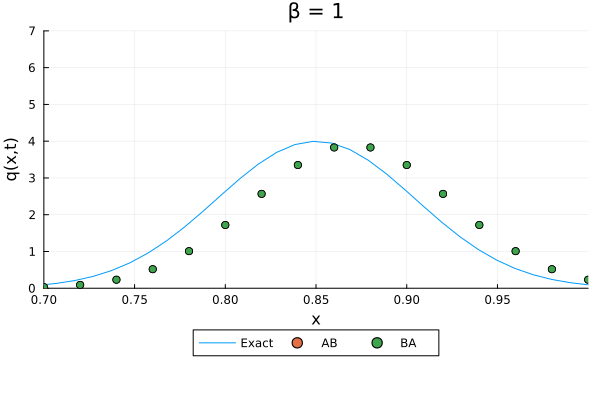
\includegraphics[width=0.5\textwidth]{Commute.png}%
		\label{fig:commute}}
	\subfloat[]{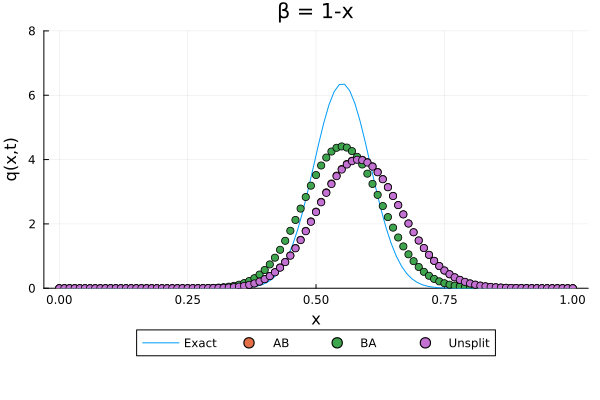
\includegraphics[width=0.5\textwidth]{NoCommute.png}%
		\label{fig:nocommute}}

	\subfloat[]{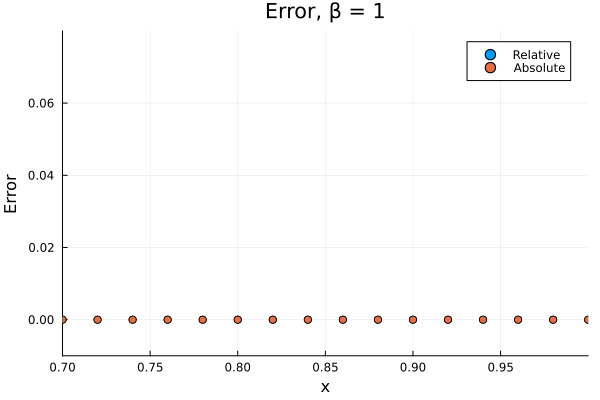
\includegraphics[width=0.5\textwidth]{CommuteErr.png}%
		\label{fig:commuteErr}}
	\subfloat[]{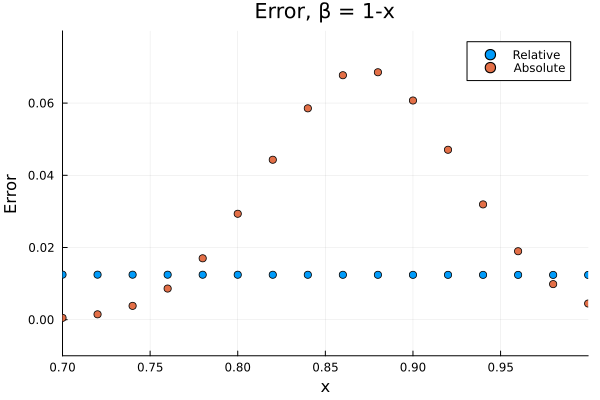
\includegraphics[width=0.5\textwidth]{NoCommuteErr.png}%
		\label{fig:nocommuteErr}}
	\caption{Comparison between the exact solution and the split method with the two different orders of steps. The difference is hardly noticeable in the plot, but the relative error is non-zero. Note that there is a big gap between the analytical  and the numerical solution because we are using a very coarse approximation to highlight the error. The problem has $\bar{u}=1$, $\mathring{q}=\text{Gaussian}(0.25,0.003)$, $\d x = \d t = 0.02$, $t=0.6$.}
	\label{fi:AB}
\end{figure*}

% possible TODO: show the offset split-unsplit method

\subsection{General Formulation}

To better understand the commuting property, we consider the more general formulation

\begin{equation}
	q_t = (\ca+\cb)q
\end{equation}

where $\ca$ and $\cb$ can be differential operators, such as $-\bar{u}\partial_x$ and $-\beta(x)$ in the case of the advection-reaction equation. To simplify the calculations, we assume that they don't explicitly depend on $t$, so that we can write

\begin{equation}
	q_{tt} = (\ca+\cb)q_t=(\ca+\cb)^2q
\end{equation}

without having to take care of the chain rule. If we Taylor expand the solution at time $t$ and use the notation defined in \eqref{eq:sol_op}, we easily get to

\begin{equation}\label{eq:exp_unsplit}
	q(x,\d t) = \sum_{j=0}^{\infty}\frac{\d t^j}{j!}(\ca + \cb)^jq(x,0) = e^{\d t(\ca +\cb)}q(x,0).
\end{equation}

With Godunov Splitting, we obtain

\begin{equation*}
	q^*(x,\d t)=e^{\d t \ca}q(x,0)
\end{equation*}

and

\begin{equation*}
	q^{**}(x,\d t)=e^{\d t \cb}q^*(x,\d t) = e^{\d t \cb}e^{\d t \ca}q(x,0).
\end{equation*}

The splitting error is then

\begin{equation}
	q(x,\d t)-q^{**}(x,\d t) = (e^{\d t(\ca +\cb)}-e^{\d t \cb}e^{\d t \ca})q(x,0).
\end{equation}

If we Taylor expand $qx^{**}$, we obtain

\begin{equation}\label{eq:exp_split}
	q^{**}(x,\d t) = (I+\d t(\ca + \cb)+\frac{1}{2}\d t^2(\ca^2+2\cb\ca+\cb^2)+\dots)q(x,0).
\end{equation}

It is fundamental to note that in the $\d t^2$ term, in \eqref{eq:exp_unsplit} we have $(\ca +\cb)^2=(\ca +\cb)(\ca +\cb)=\ca^2+\ca\cb+\cb\ca+\cb^2$, which in general is \textit{not} the same as the $(\ca^2+2\cb\ca+\cb^2)$ term that we have in \eqref{eq:exp_split}. We can clearly see now how there is no splitting error only if $\ca\cb=\cb\ca$, that is, if the operators commute. This means that if it is not the case, the Godunov method can only ever be first-order accurate, due to the splitting error.

\subsection{Strang Splitting}

\subsection{Accuracy}























\section{Implicit methods and choice of ODE solver}

In the case of Godunov splitting, we want to use a second-order accurate method in order to maintain the right accuracy. However, in general we cannot use multistep methods that require more than one level of data, because we only have $Q_i^*$ to use to compute $Q_i^{n+1}$. Values of $Q_i^*$ from previous time steps cannot be used because they are computed by solving a different problem, that is not our ODE. Runge-Kutta methods are very useful because they calculate their own intermediate values to construct higher-order approximations. For explicit methods, we need to make sure that the method is stable with the used time step.

\hfill

If the ODE $q_t=\psi(q)$ is \textit{stiff} (i.e. such that an extremely small time step is required to solve it with an explicit numerical method), as detailed in Section \ref{stiff}, then an implicit method is needed. The usual choice is the trapezoidal rule:

\begin{equation}\label{eq:trapezoidal}
	Q_i^{n+1} = Q_i^*+\frac{\d t}{2}[\psi(Q_i^*)+\psi(Q_i^{n+1})].
\end{equation}

Another nice property of the split methods is that they only require the ODE part to be solved implicitly: the hyperbolic part can still be solved with explicit methods.

If $\psi$ depends on derivatives of $q$, these need to be discretized. For example, if $\psi(q)=\mu q_{xx}$, then \eqref{eq:trapezoidal} becomes the Crank-Nicolson method and requires solving a tridiagonal system.

\section{Stiff and singular source terms and the associated numerical difficulties} \label{stiff}

The last consideration of this paper is about stiffness and singularity for source terms. Sometimes it happens that the source term is not distrbuted in space, but rather behaves like a delta function, i.e. is very large only on a small region compared to our domain. This is the case for exaple for chemical reactions that can happen on very different time scales compuared to the fluid dynamic one. If the reaction zone is concentrated, this source term is called \textit{stiff} in analogy with the the ODEs. Another typical example of stiff reacting flow is the \textit{detonation wave}: an explosion where a gas burns in a thin reaction zone and gets propagates in the rest of the gas like a shock wave. The thin reaction zone can be modeled as a delta function.

\huge DA FINIRE

% if have a single appendix:
%\appendix[Proof of the Zonklar Equations]
% or
%\appendix  % for no appendix heading
% do not use \section anymore after \appendix, only \section*
% is possibly needed

% use appendices with more than one appendix
% then use \section to start each appendix
% you must declare a \section before using any
% \subsection or using \label (\appendices by itself
% starts a section numbered zero.)
%

%\appendices
%%\section{Proof of the First Zonklar Equation}
%Appendix one text goes here.

% you can choose not to have a title for an appendix
% if you want by leaving the argument blank
%\section{}
%Appendix two text goes here.

% Can use something like this to put references on a page
% by themselves when using endfloat and the captionsoff option.
\ifCLASSOPTIONcaptionsoff
	\newpage
\fi
% trigger a \newpage just before the given reference
% number - used to balance the columns on the last page
% adjust value as needed - may need to be readjusted if
% the document is modified later
%\IEEEtriggeratref{8}
% The "triggered" command can be changed if desired:
%\IEEEtriggercmd{\enlargethispage{-5in}}

% references section

% can use a bibliography generated by BibTeX as a .bbl file
% BibTeX documentation can be easily obtained at:
% http://mirror.ctan.org/biblio/bibtex/contrib/doc/
% The IEEEtran BibTeX style support page is at:
% http://www.michaelshell.org/tex/ieeetran/bibtex/
%\bibliographystyle{IEEEtran}url

% argument is your BibTeX string definitions and bibliography database(s)
%\bibliography{IEEEabrv,../bib/paper}
%
% <OR> manually copy in the resultant .bbl file
% set second argument of \begin to the number of references
% (used to reserve space for the reference number labels box)
\begin{thebibliography}{1}

	\bibitem{leveque}
	R.~J.~LeVeque, \emph{Finite Volume Methods for Hyperbolic Problems}.\hskip 1em plus
	0.5em minus 0.4em\relax Cambridge: Cambridge University Press, 2002.

	\bibitem{github}
	\url{https://github.com/matilde-t/SeminarCourse-FundamentalsOfWaveSimulation}

	\bibitem{clawpack}
	\url{https://github.com/clawpack/apps/tree/master/fvmbook/chap17}

	\bibitem{riemann}
	\url{https://github.com/clawpack/riemann_book}

\end{thebibliography}

% that's all folks
\end{document}
